% Copyright 2007-2022 Joakim Nilsson
%
% This file is part of Combo Whist.
%
% Combo Whist is free software: you can redistribute it and/or modify
% it under the terms of the GNU General Public License as published by
% the Free Software Foundation, either version 3 of the License, or
% (at your option) any later version.
%
% Combo Whist is distributed in the hope that it will be useful,
% but WITHOUT ANY WARRANTY; without even the implied warranty of
% MERCHANTABILITY or FITNESS FOR A PARTICULAR PURPOSE.  See the
% GNU General Public License for more details.
%
% You should have received a copy of the GNU General Public License
% along with Combo Whist.  If not, see <http://www.gnu.org/licenses/>.

% Document class
\documentclass[a4paper]{article}

\usepackage[english]{babel}
% Copyright 2014-2020 Joakim Nilsson
%
% This file is part of Combo Whist.
%
% Combo Whist is free software: you can redistribute it and/or modify
% it under the terms of the GNU General Public License as published by
% the Free Software Foundation, either version 3 of the License, or
% (at your option) any later version.
%
% Combo Whist is distributed in the hope that it will be useful,
% but WITHOUT ANY WARRANTY; without even the implied warranty of
% MERCHANTABILITY or FITNESS FOR A PARTICULAR PURPOSE.  See the
% GNU General Public License for more details.
%
% You should have received a copy of the GNU General Public License
% along with Combo Whist.  If not, see <http://www.gnu.org/licenses/>.

%==========
% Packages
%==========

\usepackage[utf8]{inputenc}
\usepackage[protrusion=true]{microtype} % More readable layout
\usepackage{graphicx}                   % \rotatebox
\usepackage{tabularx}                   % X column specifier in tables
\usepackage[pass]{geometry}             % Changing margins
\usepackage[labelfont=bf]{caption}      % Captions boldface
\usepackage{siunitx}                    % Number alignment in tables
\usepackage{xfrac}                      % Vulgar fractions
\usepackage{verbatim}                   % Monospaced text
\usepackage[
	ocgcolorlinks=true,
	urlcolor={[rgb]{0,0,1}},
	linkcolor={[rgb]{0.4,0,0}},
]{hyperref}

%======================================
% Include makefile generated variables
%======================================

\input{tmp/vars.tex}

%==========
% Commands
%==========

% Rotate text 90 degrees
\newcommand{\rotccw}[1]{%
	\rotatebox{75}{{#1}}
}

\newcommand{\standardBidItem}[6]{%
	\\ \hline
	\textit{#1} &
	#2 &
	#3 &
	#4 &
	#5 &
	\small #6
}

\newcommand{\specialBidItem}[4]{%
	\\ \hline
	\textit{#1} &
	#2 &
	\raggedright\textit{#3} &
	\small #4
}

\newcommand{\nonTrump}{\textnormal{non-trump bids}}

\newcommand{\introPages}{%
	\maketitle

	\vfill

	% Logo
	\begin{center}
		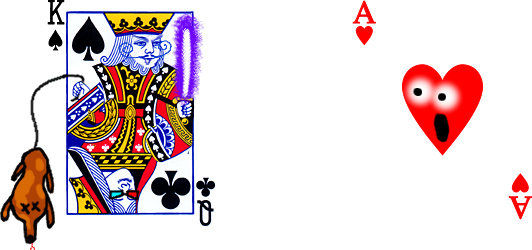
\includegraphics[width = \textwidth]{../logo.png}
	\end{center}

	\vfill

	% License
	% This file is part of Combo Whist.
%
% Copyright 2014-2019 Joakim Nilsson
%
% This file is part of Combo Whist.
%
% Combo Whist is free software: you can redistribute it and/or modify
% it under the terms of the GNU General Public License as published by
% the Free Software Foundation, either version 3 of the License, or
% (at your option) any later version.
%
% Combo Whist is distributed in the hope that it will be useful,
% but WITHOUT ANY WARRANTY; without even the implied warranty of
% MERCHANTABILITY or FITNESS FOR A PARTICULAR PURPOSE.  See the
% GNU General Public License for more details.
%
% You should have received a copy of the GNU General Public License
% along with this text.  If not, see <http://www.gnu.org/licenses/>.
% License notice

\begin{verbatim}
	Copyright 2007-2019 Joakim Nilsson

	This document is part of Combo Whist.

	Combo Whist is free software: you can redistribute it and/or modify
	it under the terms of the GNU General Public License as published by
	the Free Software Foundation, either version 3 of the License, or
	(at your option) any later version.

	Combo Whist is distributed in the hope that it will be useful,
	but WITHOUT ANY WARRANTY; without even the implied warranty of
	MERCHANTABILITY or FITNESS FOR A PARTICULAR PURPOSE.  See the
	GNU General Public License for more details.
\end{verbatim}
\verb|You should have received a copy of the GNU General Public License|\\
\verb|along with this text.  If not, see <|\url{http://www.gnu.org/licenses/}\verb|>.|


	\thispagestyle{empty}
	\pagebreak

	% Table of contents and list of tables without protrusion
	\microtypesetup{protrusion=false}
	\setcounter{tocdepth}{3}
	\tableofcontents
	\listoftables
	\microtypesetup{protrusion=true}
	\thispagestyle{empty}
	\pagebreak
}


% Title
\defTitle{Combo Whist}{The Taintless Card Game}

% Links text
\defLinks{For the latest version of the rules, visit \rulesUrl, or subscribe to \rssUrl.}

% Author
\author{By Joakim Nilsson}

% Date and version
\ifdefined\varDev
	\date{Development version (based on version \varVersion-\varLanguage)---\today}
\else
	\date{Version \varVersion-\varLanguage\---\today}
\fi

% Document
\begin{document}
	%=============
	% Intro pages
	%=============

	\introPages
	\pagebreak

	%======
	% Body
	%======

	\section{Overview}
		Combo Whist is a trick-taking card game and is---as its name implies---a variant of Whist. The key trait of Combo Whist is its great variety of available strategies while still having a rule set that is fairly simple (although the rule set is undeniably somewhat large). The possibility for many and varied strategies avoids a substantial amount of randomness that is usually present in Whist games, without making the game overly complicated, keeping it fun to play for both experienced and casual card players.

		\paragraph{Number of players:}
			Preferably 4, but 3 to $\infty$ is also possible with some adjustments to the rules.

		\paragraph{Requirements:}
			A standard 52 card deck, a pen and a piece of paper.

		\paragraph{Card rank:}
			From highest to lowest: A, K, Q, J, 10, 9, 8, 7, 6, 5, 4, 3, 2

	\section{How to play}
		\subsection{Preparations}
			Make a column for each player on the paper. This is for keeping track of each players' score as well as some other information about the game. After you have properly prepared the paper, choose a dealer at random.

			If there are only 3 players, $\clubsuit 7$, as well as all the 8s, 9s and 10s are removed from the deck.

		\subsection{Deal}
			There are two main parts of a deal. The first part is the \emph{bidding} and the second part is the \emph{game}. Because things should be easier to understand in the reverse order, the game is described before the bidding.

			A deal begins with the dealer dealing 13 cards to each player. Next, the bidding begins and when it has finished, the game begins.

			After the game, players' new scores are noted down and a new deal begins with the next dealer being the player who is seated to the left of the current dealer.

			\subsubsection{Game}
				The game plays similarly to any Whist variant. The player to the right of the \emph{declarer}\footnote{The term ``declarer'' is explained in Section~\sectionref{bidding}.} leads by playing a card. Next, the player to the left of them plays a card which must follow the suit of the first card. After that, the next player (one step further left) plays yet another card which must also follow the suit of the first card, and so on until all players have played one card each.

				If a player is out of cards in the leading suit, they may discard any card or play a trump. Unlike many variants of Whist, it is not mandatory to play a trump in case one would be out of cards in the leading suit.

				The player who played the highest card in the leading suit takes the \emph{trick} (that is, takes all the played cards and puts them face-down on the table) unless a trump is played, in which case the player who played the highest trump takes the trick. The player who brought home the last trick leads the next one.

			\subsubsection{Bidding}
				\label{sec:bidding}
				In Combo Whist, players make \emph{combo bids}. A combo bid is composed of exactly one standard bid and any amount (including zero) of unique special bids. The bids have certain rules associated with them that are applied during the game and during scoring.

				The players take turns by bidding in a clockwise manner and the player to the left of the dealer makes the first bid. A player can either pass or make a combo bid that is worth more than the previous combo bids (from here on simply referred to as \emph{bids}). If a player passes, they are out of the bidding and may therefore not make any new bids until the next deal. If all players pass, the same dealer collects all cards and deals a new deal.

				A bid's worth is defined as the combined worth of the standard and special bids it comprises. A bid must have a worth of least 1 in order for it to be eligible for bidding. A proposed time limit between bids is 20 seconds, but 1 minute before the initial bid. Although for beginners higher limits or no limits are recommended. If a player hasn't made a bid within the given time limit, they automatically pass. The bidding continues until all players but one have passed. That player is appointed declarer and the game begins.

				The available bids are listed in the tables in Section~\sectionref{standardBids} and Section~\sectionref{specialBids}. The number of tricks to bring home in order to complete the bid is listed in the standard bids table in the ``Tricks'' column. A special bid cannot be combined with another bid listed in the ``Incompatibility'' column, nor are combo bids allowed which are impossible to complete regardless of the distribution of the cards of the opponents. Note that there is a difference between worth and score; Worth is a bid's worth (You guessed it!) and score is the number of points the declarer scores if they complete a bid.

				If it is unclear when an event triggered by a bid is supposed to occur, refer to the special bids' ``Order'' column. The order of a bid decides in what order the events given by its rules will take place. The bids with the lowest order go first. All of the standard bids have order 0.

			\subsubsection{Scoring}
				After the game has finished, the declarer scores a number of points determined by what combo bid was bid and whether it was completed. If the bid was completed, they score as many points as as noted in the ``Score'' column for the standard bid. If the bid was not completed, 2 points are subtracted from their previous score. It is possible to attain a negative score. If a player has a score below $-5$, they are not allowed to bid during bidding. However, they automatically score 1 point for free after every deal they participate in (even if no one bids).

			\subsubsection{Winning}
				\label{sec:winning}
				There are two variants on how to determine the winner in Combo Whist: \emph{classic} and \emph{limited}.

				\paragraph{Classic:}
				The winner is the player who first attains or exceeds the \emph{winning score}. The winning score starts at 13, but 1 is subtracted from it every time all players have dealt one deal each. The winning score decreases \emph{after} the final deal has been completed and scores for that deal have been counted. This continues until the winning score reaches 1. A player must win by completing a bid and can therefore not win merely because the winning score just decreased. A player can also not win unless they have the solitary highest score.

				\paragraph{Limited:}
				A predetermined number of \emph{rounds} are played (one suggestion is 3), where one round comprises each player dealing one deal each. When the rounds have been played, the next player wins who completes a bid which results in that said player attains the solitary highest score. To clarify: A player can win when the last round is completed.

				\paragraph{Win of Shame:}
				Common to both variants is the following rule: If all players but one attains a score of $-5$ or lower, the player who has the higher score automatically wins, regardless of the winning score. This type of win is called a \emph{Win of Shame}.

	\section{Miscellaneous}
		\subsection{Rules for more than 4 players}
			If there are more than 4 players participating in the game, for every deal, all players but 4 sit out (that is, they don't participate in the deal). These players are the ones that are closest to the right of the dealer.
		
		\subsection{Talking}
			A certain amount of talk is allowed in Combo Whist, but the players are not allowed to give hints about what cards they have.
		
		\subsection{Cheating}
			If the declarer unintentionally cheats, the current bid is not completed. If a non-declarer unintentionally cheats, the following occurs: The current bid continues, but no subtraction of points is done from the declarer's score should the bid not be completed. Furthermore, the same amount of points as the current bid's points is subtracted from the cheating player's score regardless of whether the bid is completed.
			
			If unintentional cheating occurs before a declarer has been appointed, the deal is canceled, and 2 points are subtracted from the cheating player's score.

			However, if all of the deal's players agree about how the events after the cheating occured should be reversed, they should be reversed in the agreed-upon manner, without other changes to the scores except that 1 point is subtracted from the cheating player's score.

			A player who intentionally cheats in Combo Whist is never again allowed to play it because they obviously do not respect the game's magnificence.

	%============
	% Bid tables
	%============

	\pagebreak
	\newgeometry{left=1cm, right=1cm, top=1cm}

	\section{Standard bids}
		\label{sec:standardBids}
		\begin{center}
			\begin{tabularx}{\textwidth}{
					p{2.5cm}
					S
					S
					ccX
				}

				\textbf{D\scriptsize ESIGNATION} &
				\rotccw{\textbf{Worth}} &
				\rotccw{\textbf{Score}} &
				\rotccw{\textbf{Trump}} &
				\rotccw{\textbf{Tricks}} &
				\textbf{Rules}
				\\[-3ex]

				\directlua{tableItemsStandardBids()}
			\end{tabularx}
		\end{center}

	\newcommand{\nonTrump}{\textnormal{trumpless bids}}
	\section{Special bids}
		\label{sec:specialBids}
		\begin{center}
			\begin{tabularx}{\textwidth}{
					p{2.3cm}
					S
					S
					p{2.7cm}
					X
				}

				\textbf{D\scriptsize ESIGNATION} &
				\rotccw{\textbf{Worth}} &
				\rotccw{\textbf{Order}} &
				\textbf{Incompatibility} &
				\textbf{Rules}
				\\[-3ex]

				\directlua{tableItemsSpecialBids()}
			\end{tabularx}
		\end{center}
\end{document}
